\usepackage{fancyhdr}\documentclass[conference]{IEEEtran}
\IEEEoverridecommandlockouts
% The preceding line is only needed to identify funding in the first footnote. If that is unneeded, please comment it out.
\usepackage{cite}
\usepackage{amsmath,amssymb,amsfonts}
\usepackage{algorithmic}
\usepackage{graphicx}
\usepackage{textcomp}
\usepackage{xcolor}
\usepackage{hyperref}
\usepackage{tikz}
\usepackage{subfigure}
\def\BibTeX{{\rm B\kern-.05em{\sc i\kern-.025em b}\kern-.08em
    T\kern-.1667em\lower.7ex\hbox{E}\kern-.125emX}}
\begin{document}

\title{\huge Stock Price Prediction Using Machine Learning Algorithms}

\author{\IEEEauthorblockN{Kate Catalena}
\IEEEauthorblockA{\textit{UIN: 421003524} }
\and
\IEEEauthorblockN{Zebo Xiong}
\IEEEauthorblockA{\textit{UIN: 128007734}}
\and
\IEEEauthorblockN{Mohd Faisal Khan}
\IEEEauthorblockA{\textit{UIN: 727006629}}
\and
\IEEEauthorblockN{Nader Ghasemi}
\IEEEauthorblockA{\textit{UIN: 121002001}}
}

\maketitle

\begin{abstract}
Predicting stock market trends has been and still is a very popular area of research. Stock market prices
represent changes in the economy. Many factors go into determining what a stock market price will do in the
future, which makes predicting future trends nearly impossible. There is a lot of machine learning research
devoted to this idea because if you can identify underlying trends, you can better anticipate
what a stock market price will do down the road. In this research, we plan to take a survey of current machine
learning techniques and apply them to financial data to analyze which techniques perform better in terms
of predicting future stocks. A survey of the most commonly used methods and how well they perform on
the same data set would be useful in understanding each method, including their strengths, weaknesses, and
overall performance in predicting future stocks. We have collected hourly data for Apple Stock since the year 2004. We hope that with hourly data, we report a better accuracy rate than other papers who have only used daily data. 
\end{abstract}

\begin{IEEEkeywords}
\\ 
\\
Machine Learning, Stocks, SVR, SVM, LTSM, XGBoost
\end{IEEEkeywords}

\section{Introduction}
Predicting stock market trends is difficult due to the fact that they vary in response to many external features. The external features that can affect stock market prices range from economical, political, and  international just to name a few. This is one of the main reasons predicting stock market trends is so complicated. There are so many external features, it is hard to gather the data and use that data in models. 
\begin{figure}[h]
    \centering
    {
        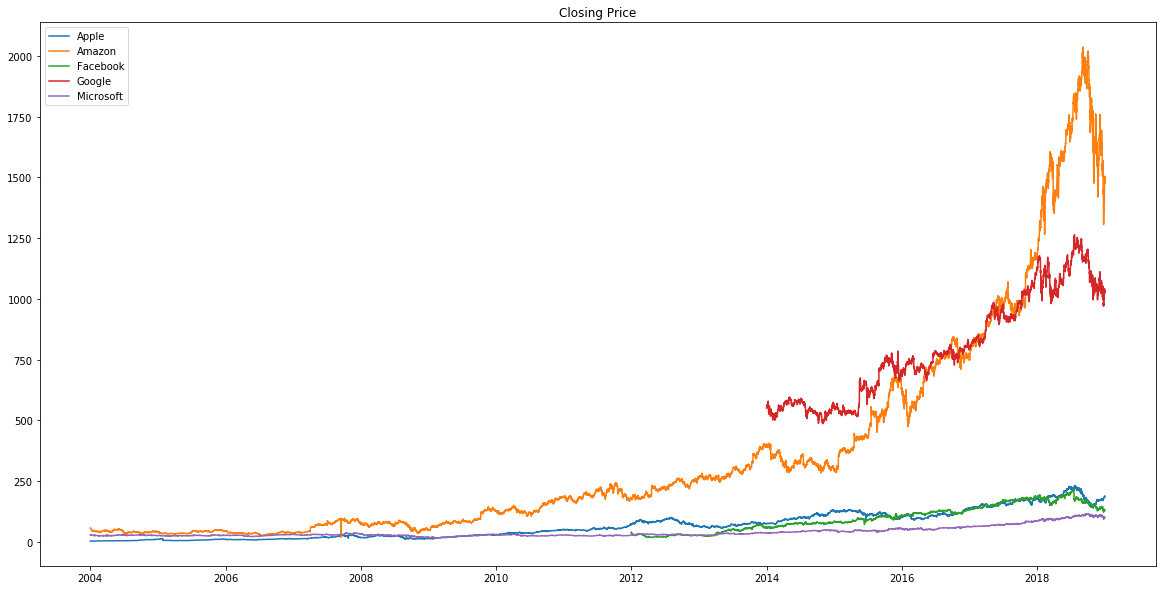
\includegraphics[width=3.0in]{all_data.png}
        \label{fig:first_sub}
    }
    \caption{Variation of Stock prices of Big5 from 2004}
    \label{fig:sample_subfigures}
\end{figure}
\\
\\

Much of the work related to this paper built their models using daily data. We have acquired hourly data for the Apple stock. We expect that having the hourly data will produce better results than those found in other papers. We have chosen to implement an SVR, SVM, XGBoost, and LTSM. We have chosen these because SVR and SVM are simpler algorithms compared to XGBoost and LTSM. 
\\
\section{Related Work}
In previous studies, the features selected for the inputs to the machine learning algorithms are mostly derived from the data within the same market under concern. Such isolation leaves out important information carried by other entities and make the prediction result more vulnerable to local perturbations.\\ \\
   Efforts have been done to break the boundaries by incorporating external information through fresh financial news or personal internet posts such as Twitter. These approaches, known as sentiment analysis, replies on the attitudes of several key figures or successful analysts in the markets to interpolate the minds of general investors. Recently, no financial market is isolated. Economic data, political perturbation and any other oversea affairs could cause dramatic fluctuation in domestic markets.  \\  \\
   We also propose the use of global stock data in associate with data of other financial products as the input features to machine learning algorithms such as SVM. In particular, we are interested in the correlation between the closing prices of the markets that stop trading right before or at the beginning of US markets. Oversea markets that closes right before or at the beginning of the US market trading should provide valuable information on the trend of coming US trading hour, as their movements already account for possible market sentiment on latest economic news or response to progress in major world affairs. \\ \\
   Commodity prices & foreign currency data are also listed as potential features, as different financial markets are interconnected. For instance, slowdown in US economy will definitely cause a drop in US stock market. But at the same time, USD and JPY will increase with respect to its peers as people seek for asset havens. Such interplay implies the underlying relationship between these financial products and the possibility of using one or some of them to predict the move of the other ones\\
\\ \\
Leong et al. looked at incorporating a support vector
machine to predict movements in future stock prices \cite{1}. To solve the SVM optimization problem, they
used minimum graph cuts, which allowed their SVM to better predict more complex tree structures. With
a 3-fold cross-validation method, they were able to achieve 78\% accuracy with their SVM, which indicates
their model was successful in learning and predicting future stock market prices without overfitting. Huang et al. used a neural-network method to better predict Chinese stock prices. More specifically, they used a
Bayesian-LTSM neural network method \cite{2}. They use six indicators for input into their LTSM. For their
data, they looked at 26 years’ worth of data and then broke down each year into a week. With this model,
they reported that, on average, their Bayesian-LTSM predicted stock market prices 25 percent better than a
regular LTSM approach.

\section{DATA SELECTION AND IMPLEMENTATION}
For the purpose of this research we have implemented four different machine learning algorithms: SVR, SVM, XGBoost, and LTSM. We chose these algorithms because they range from fairly simply (SVR and SVM) to more complicated (XGBoost and LTSM). We felt this would give us deep understanding of how different models perform and work on the data. It would also give insight into overall performance, weaknesses, and strengths.
\\



\subsection{XGBoost}
XGBoost stands for Extreme Gradient Boosting. It implements the Machine Learning Algorithms using Gradient Boosting. This is an ensemble method and applies the principle of Boosting weak learners. XGboost approaches the process of building sequential tree using parallel implementation. For pruning the tree it uses multiple parameters described.\\
\begin{figure}[h]
    \centering
    {
        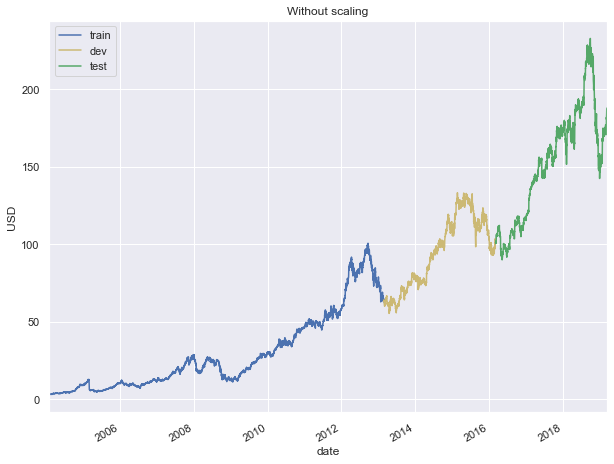
\includegraphics[width=3.0in]{partition.png}
        \label{fig:first_sub}
    }
    \caption{Splitting the data, 60\% training, 20\% cross validation, 20\% testing}
    \label{fig:sample_subfigures}
\end{figure}
\subsubsection{Feature Selection}
The input data consisted of Parameters: Open Price, Close Price, High Price, Low Price, Weighted Avg. Price, Volume Traded. We focused on the 'APPLE' hourly data for the stock prices from the year 2004 to 2019. Using the aforementioned parameters, we constructed following features for training the model. The features are\cite{5}:\\
- High Price - Low Price\\
- Open Price - Close Price\\
- Rolling Mean for 7 previous Hours.\\
- Rolling Standard deviation for 7 previous Hours.\\
\\
Post the feature construction we scaled and partitioned the data into training, validation and testing dataset in the ratio 60:20:20 as shown in Fig 2.\\

\subsubsection{Hyper-Parameter Tuning}
XGBoost has the following hyper parameters: Learning Rate, Gamma, Max Depth of Tree, Min Child Weight, Number of Estimators, colsample by tree, colsample by level, etc\cite{7}. We trained the model on the training data and tuned the hyper-parameters by using multiple values and calculating the RMSE for each case on the validation data. The final model to be tested uses the optimum tuned hyper-parameters\cite{6}. Fig 3. Shows the variation of RMSE for different hyper-Parameters value.
\begin{figure}[h]
    \centering
    \subfigure[Gamma]
    {
        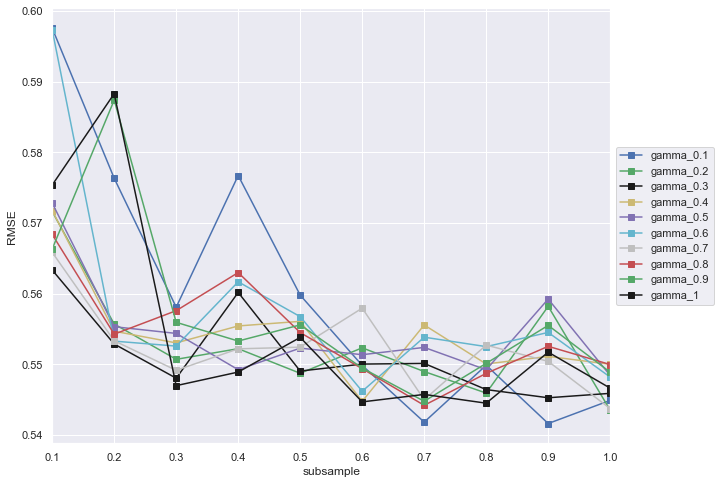
\includegraphics[width=1.5in]{gamma.png}
        \label{fig:first_sub}
    }
    \subfigure[Max Depth]
    {
        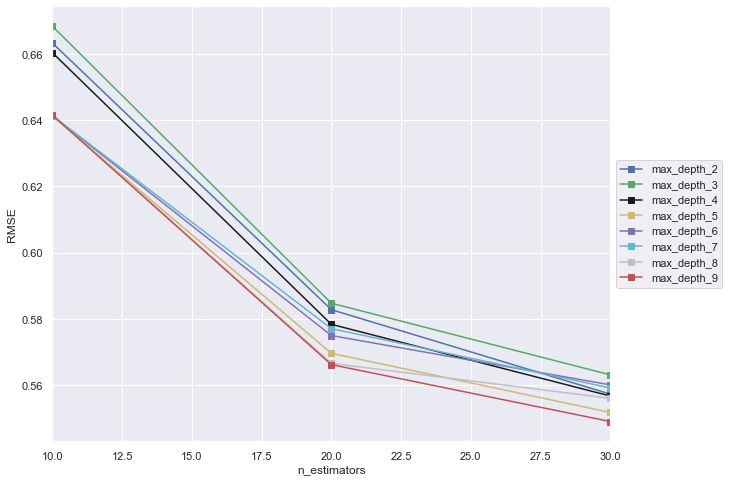
\includegraphics[width=1.5in]{max_depth.png}
        \label{fig:second_sub}
    }
    \\
    \subfigure[Colsample by Level]
    {
        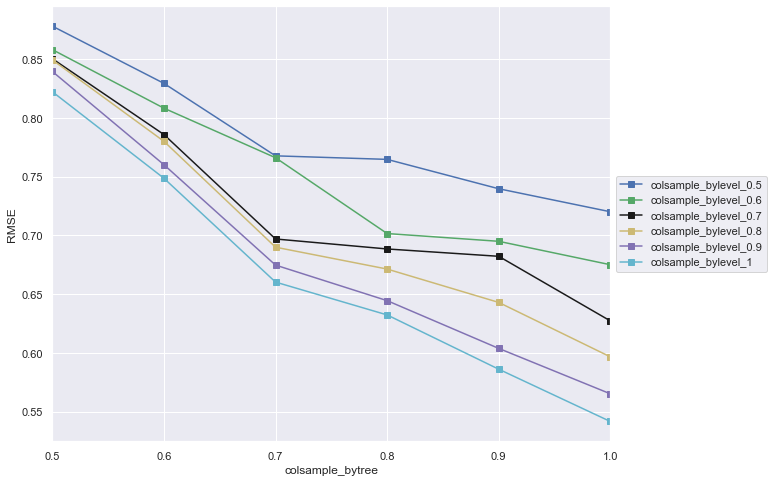
\includegraphics[width=1.5in]{colsample.png}
        \label{fig:third_sub}
    }
    \subfigure[Min Child Weight]
    {
        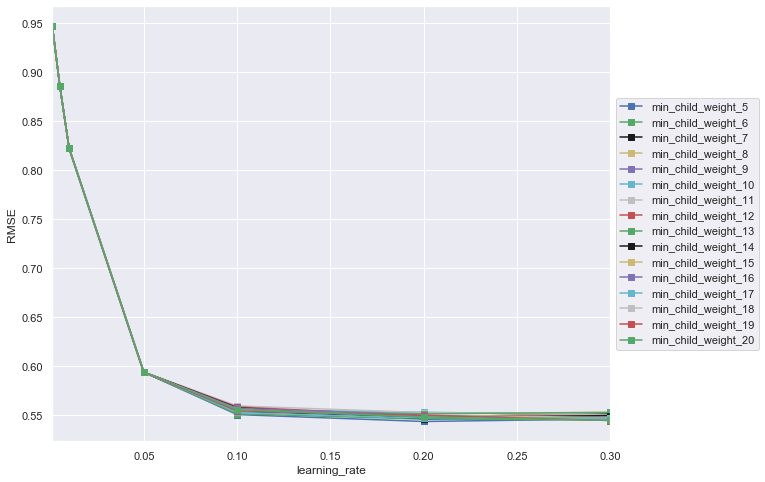
\includegraphics[width=1.5in]{min_child_weight.png}
        \label{fig:fourth_sub}
    }
    \caption{Optimizing Hyperparameters}
    \label{fig:sample_subfigures}
\end{figure}
\begin{table}[h]
\renewcommand{\arraystretch}{1.3}
\caption{Calculated Metrics (XGBoost)}
\label{tab:example}
\centering
\begin{tabular}{|c|c|c|c|c|c|}
    \hline
    Stocks  &  RMSE & MSE & MAE & MAPE(\%) & R2 Score\\
    \hline
    \hline
    Apple   &   0.837 & 0.7 & 0.474 & 0.305 & 0.99\\
    \hline
    Facebook   &   1.397 & 1.95 & 0.73 & 0.434 & 0.99\\
    \hline
    Google   &   6.662 & 44.38 & 4.56 & 0.417 & 0.99\\
    \hline
    Amazon   &   8.398 & 70.52 & 4.42 & 0.384 & 0.99\\
    \hline
    Microsoft   &   0.383 & 0.146 & 0.225 & 0.288 & 0.99\\
    \hline
\end{tabular}
\end{table}
\\
\begin{figure}[h]
    \centering
    \subfigure[Histogram of Residuals]
    {
        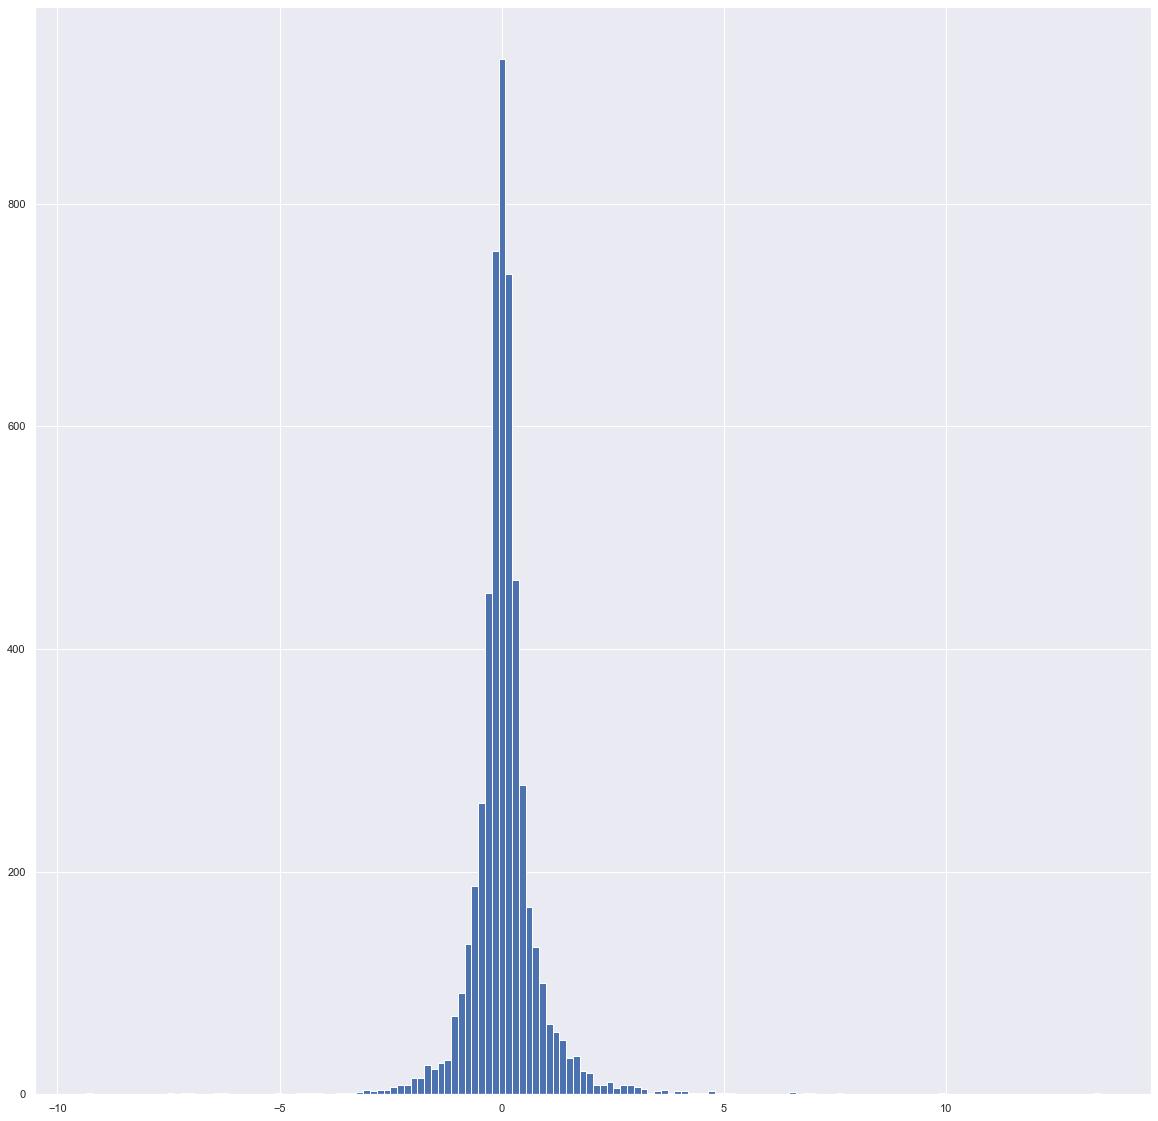
\includegraphics[width=1.5in]{hist.png}
        \label{fig:first_sub}
    }
    \subfigure[Residual vs Fitted values]
    {
        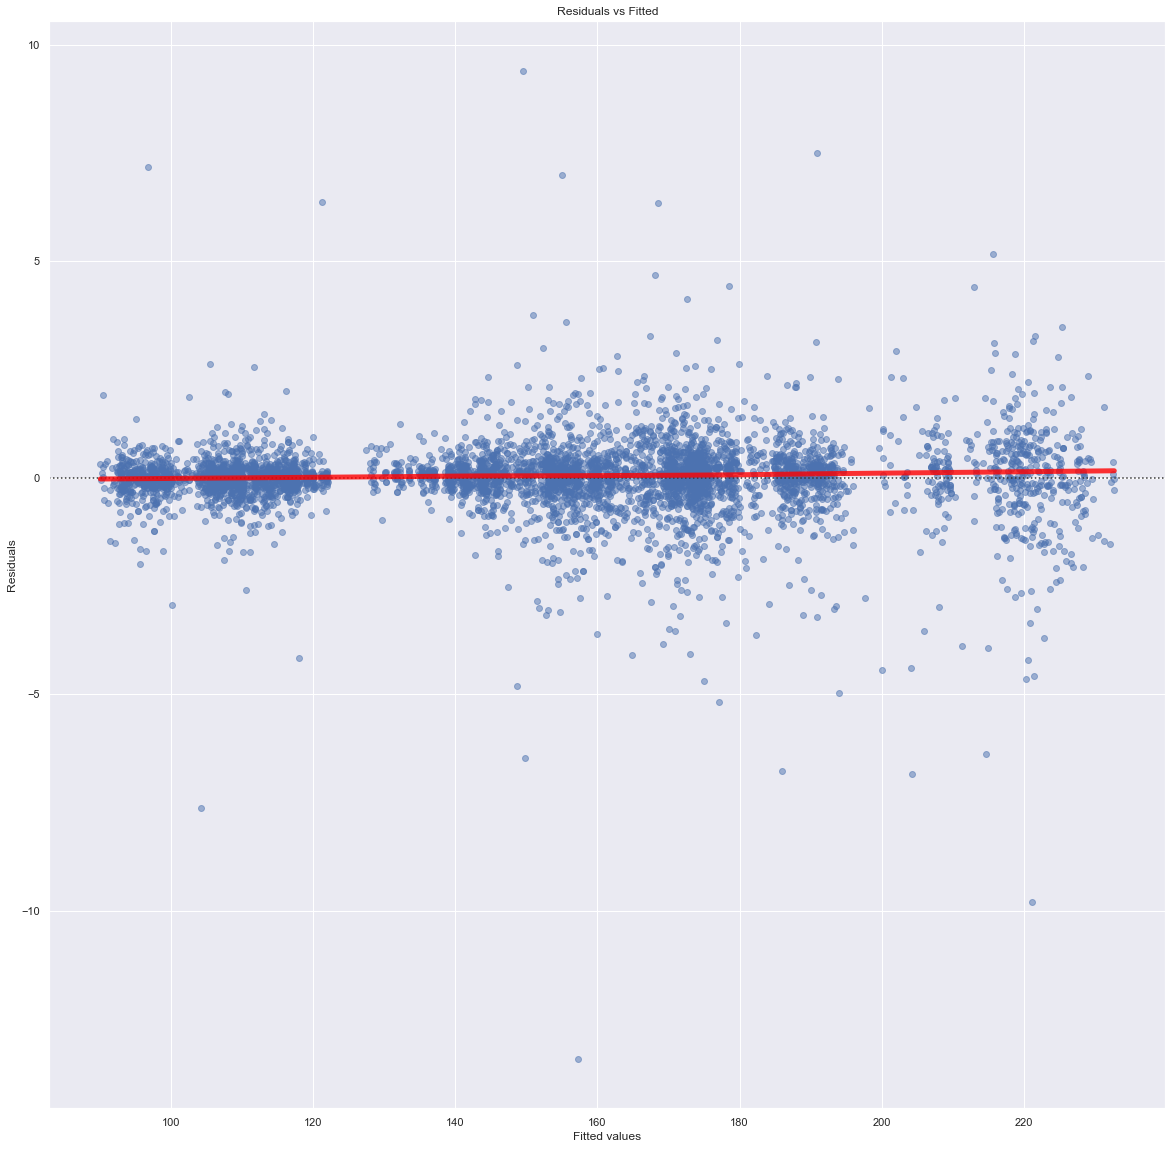
\includegraphics[width=1.5in]{residuals.png}
        \label{fig:second_sub}
    }
    \caption{Plotting Residuals}
    \label{fig:sample_subfigures}
\end{figure}
\subsubsection{Observation}
The model was trained and tested for all the Big5 tech stock companies and the Table 1 shows the calculated metrics observed. XGBoost, in spite of being a tree based model captured the data quite well. However in case of Amazon and Google, we can see from the table the values are higher than other companies. This can be explained from the fact that the trend in Amazon changed drastically throughout these years. For Google we had data only for 5 years compared to the 15 years data for the other stocks.

\\
To check the performance of XGBRegressor, we also plotted the residual Histogram plot and Residual vs Fitted Values (Fig 4). From Fig 4(a), we observed that the residual follow a normal distribution and Fig 4(b) tells that the residuals are close to the mean value of zero throughout the data cycle. Hence we can establish that the XGBregressor model performed pretty well.


\subsection{Support Vector Regression (SVR)}
SVRs are similar to SVCs. They use a support vector machine in order to train a model, but instead of using classification, regression is used. Predicting stocks, or any numerical result, is very difficult because there are an infinite number of possibilities. When dealing with stocks, we face complications because the data is not linear. Non-linear data tends to be much more difficult to work with. We can implement a Polynomial kernel or a Radial Basis Function kernel in order to transform our non-linear data to a high dimensional vector space so the data is easier to work with. Figure 3 represents the transformation from a non-linear data set to a linear data set in a high dimensional vector space\cite{3}. 
\\
\begin{figure}[h]
    \centering
    \subfigure
    {
        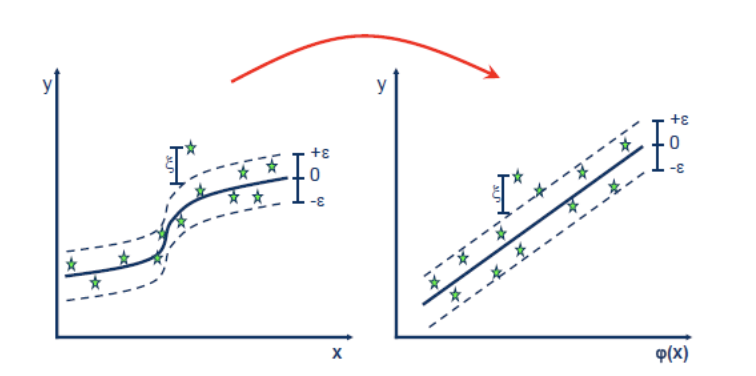
\includegraphics[width=2.0in]{nonlin.png}
        \label{fig:first_sub}
    }
    \caption{Transformation of non-linear data to a high-dimensional vector space}
    \label{fig:sample_subfigures}
\end{figure}
\\
We have chosen to use an RBF kernel. There are two parameters that we focus on for an RBF kernel: C and  γ. The C parameter is a trade off between finding the correct value of the training examples and the maximization of the decision function’s margin \cite{4}. The higher the C value, the more likely the model is over fitting. γ is the influence a single training example has on the model\cite{4}. Similar to the C parameter, the larger the γ value, the more likely the model is over fitting. 
\subsubsection{Feature Selection}
For the SVR model, we used the same features described above in the XGBoost section.
\\
\\
\subsubsection{Optimization of Parameters}
In order to identify what the best parameters would be, we trained the model for varying values of C and $\gamma$. We then used the trained model to predict the validation set in order to identify which combination minimized the loss functions. We used several C and $\gamma$ values ranging from $2^{-3}$ up to $2^8$. Figure 4 represents how the loss functions changed when varying the C and $\gamma$ parameters. It turns out that a C value of 1/8 and a $\gamma$ value of 1/2 produced the best model. We trained and tested 64 different models on the validation set in order to determine these parameters. Training and testing 64 different parameters took a good bit of time, approximately 1 hour and 15 minutes. 
\\
\\

\subsubsection{Observations}
After identifying the optimal C and $\gamma$ parameters, we ran the model on the Apple, Facebook, Amazon, Google, and Microsoft stock test data sets. Although optimizing the parameters took a lot of time, running the models did not take long at all. They each ran under 20 seconds.  Table 2 shows the loss functions and $R^2$ metrics for both sets of data. Figure 4 shows the prediction on the test data given by the model. 
\\
\\
\begin{figure}[h]
    \centering
    \subfigure[RMSE]
    {
        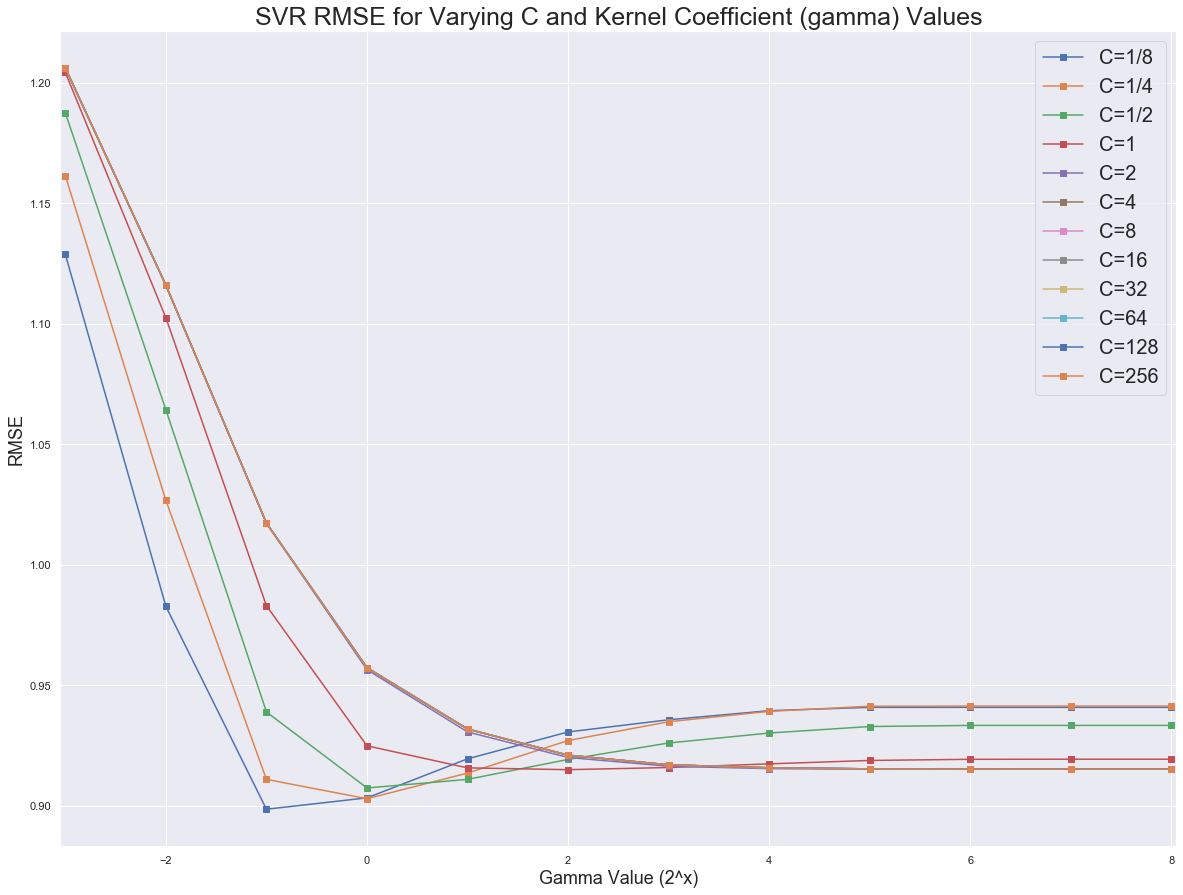
\includegraphics[width=1.5in]{svr_rmse.png}
        \label{fig:first_sub}
    }
    \subfigure[MAPE]
    {
        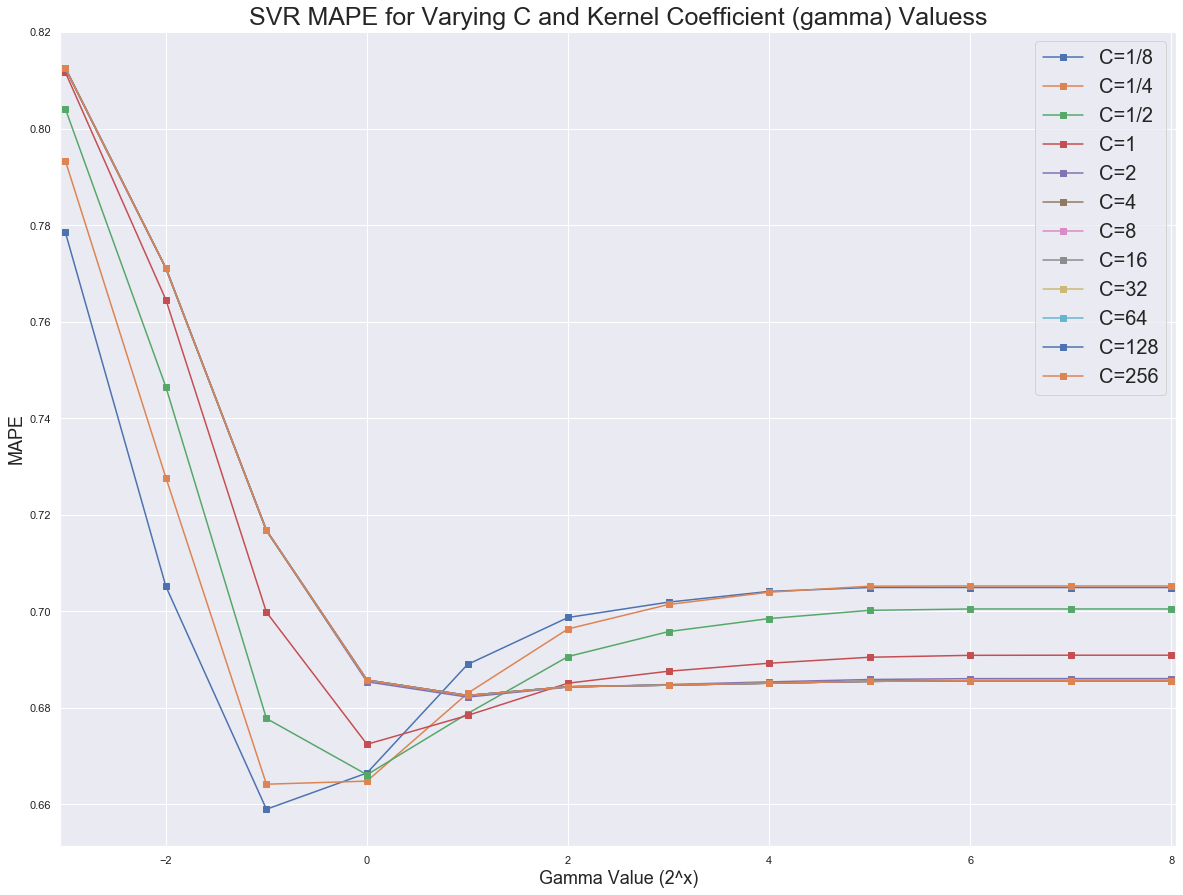
\includegraphics[width=1.5in]{svr_mape.png}
        \label{fig:second_sub}
    }
    \\
    \subfigure[MSE]
    {
        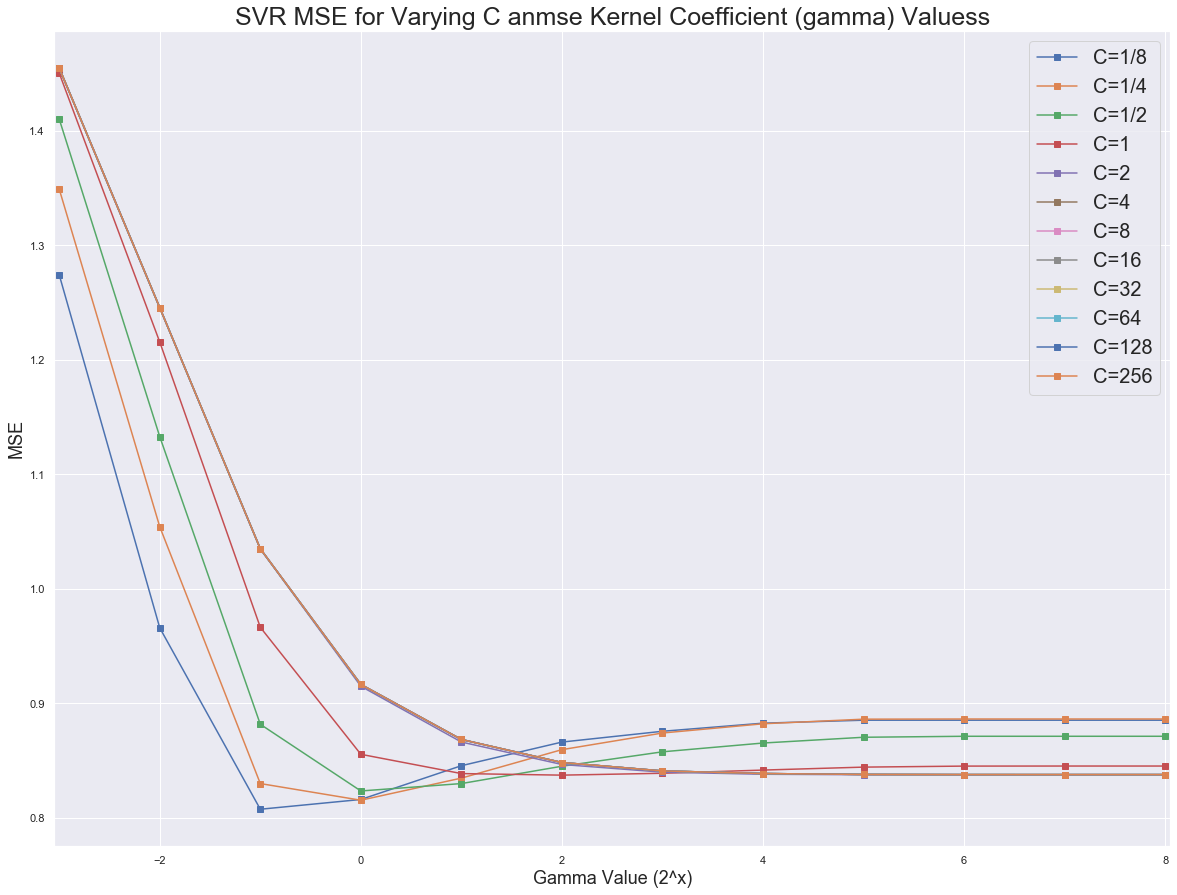
\includegraphics[width=1.5in]{svr_mse.png}
        \label{fig:third_sub}
    }
    \subfigure[MAE]
    {
        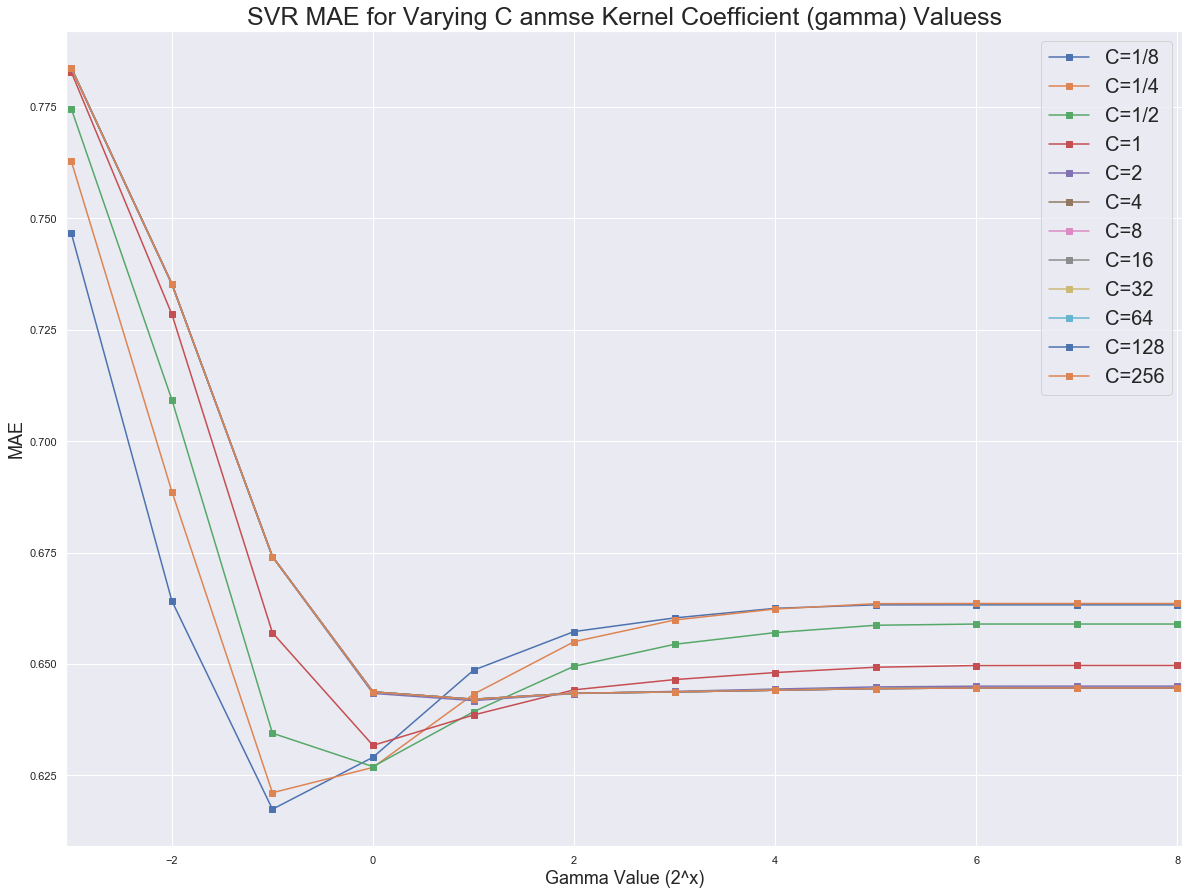
\includegraphics[width=1.5in]{svr_mae.png}
        \label{fig:fourth_sub}
    }
    \caption{Optimizing C and $\gamma$ by minimizing loss functions}
    \label{fig:sample_subfigures}
\end{figure}
\\
\\
We can see from the table, that the SVR model did decently well. We tuned our model using the Apple stock information and then used those parameters in order to train and test on the other stock companies. The loss functions were the smallest for Apple, Facebook, and Microsoft, which makes sense considering we had more data to train our models on and these three stocks are quite stable for the entire time period. The Google and Amazon data is more varied, and there was less data to train on. Overall, SVR is a quick method, that once tuned can perform relatively well for stock prediction. 

\\


\begin{table}[h]
\renewcommand{\arraystretch}{1.3}
\caption{Calculated Metrics (SVR)}
\label{tab:example}
\centering


\begin{tabular}{|c|c|c|c|c|c|}
    \hline
    Stocks  &  RMSE & MSE & MAE & MAPE(\%) & R2 Score\\
    \hline
    \hline

    Apple   &   1.468 & 2.154 & 0.9351 & 0.6018 & 0.9983\\
    \hline

    Facebook   &   2.4062 & 5.7898 & 1.4136 & 0.8412 & 0.9806\\
    \hline

    Google   &  11.7110  & 137.148 & 8.6434  & 0.7866  & 0.9702\\
    \hline
  
    Amazon   &  14.9153  & 222.4661  & 8.5438 & 0.7433 & 0.99874\\
    \hline
    
    Microsoft   &  2.4062  & 5.7898 & 1.4136 & 0.8412 & 0.9806\\
    \hline
\end{tabular}

\end{table}



\begin{figure}[h]
    \centering
    \subfigure[Apple]
    {
        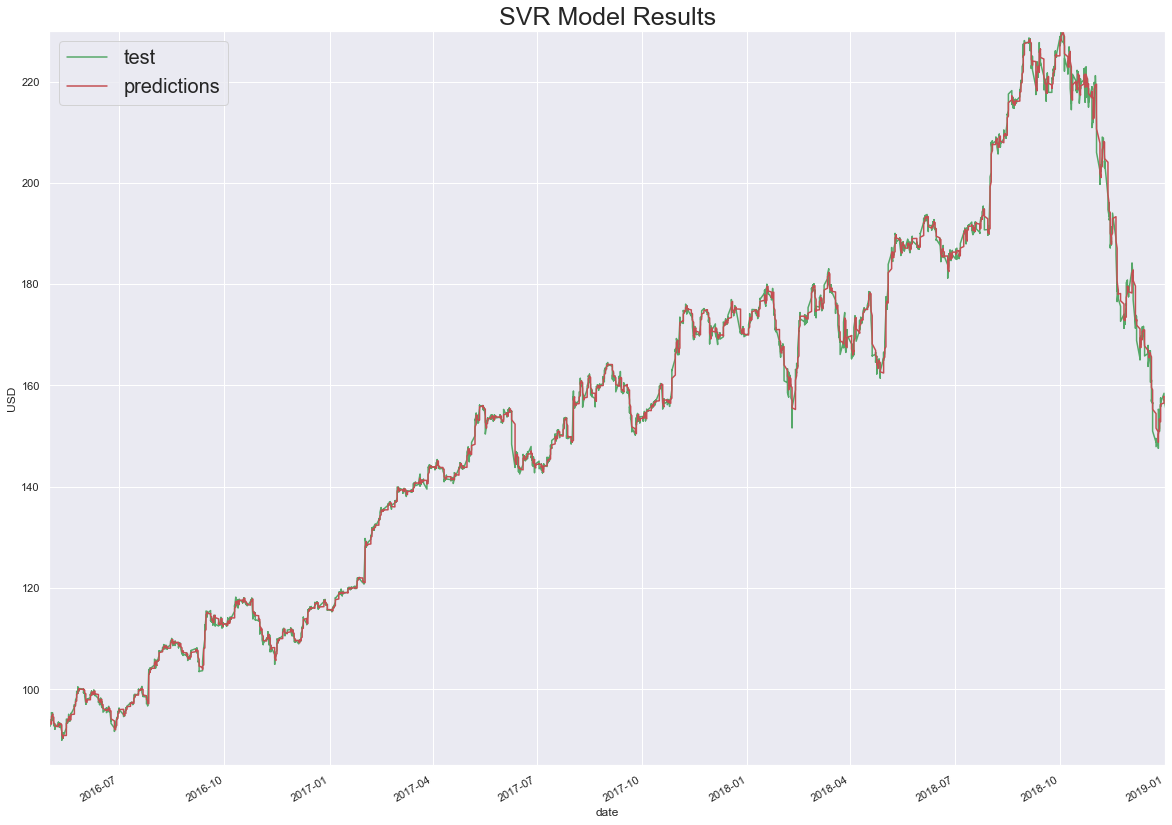
\includegraphics[width=1.5in]{apple_test.png}
        \label{fig:first_sub}
    }
    \subfigure[Facebook]
    {
        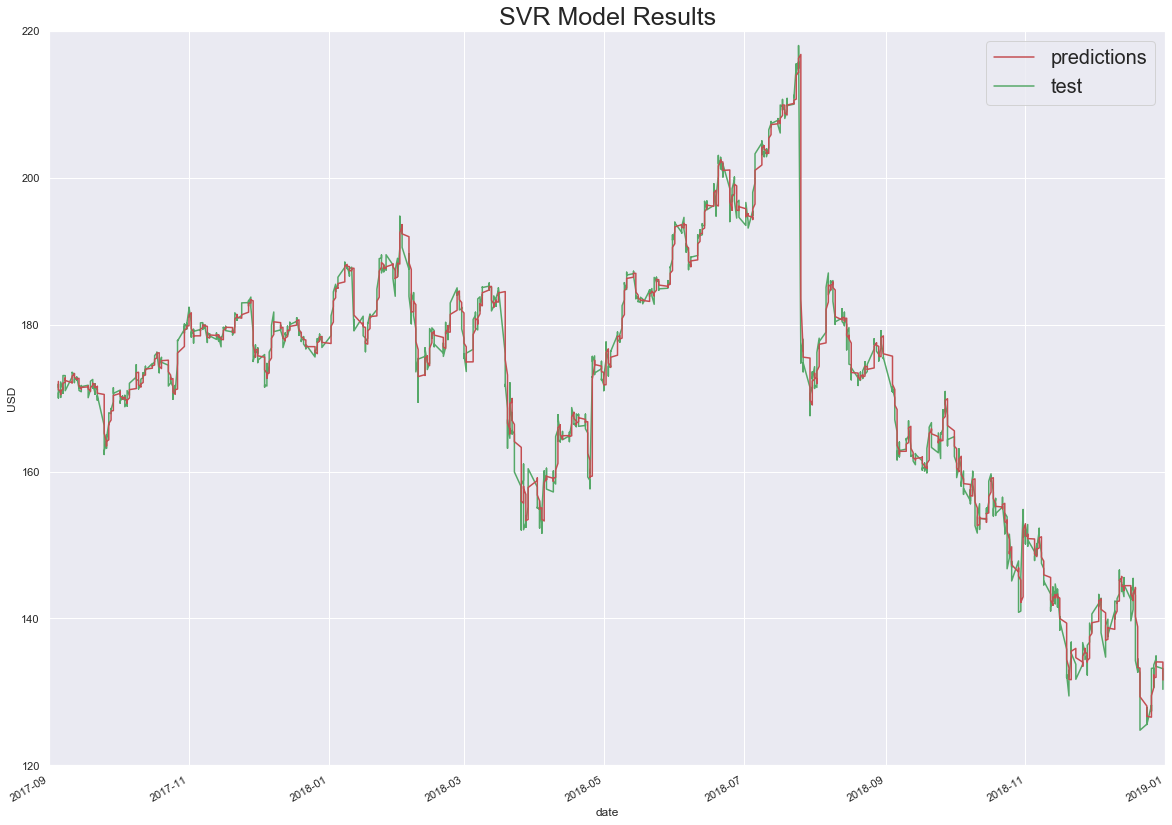
\includegraphics[width=1.5in]{facebook_test.png}
        \label{fig:second_sub}
    }
    \subfigure[Amazon]
    {
        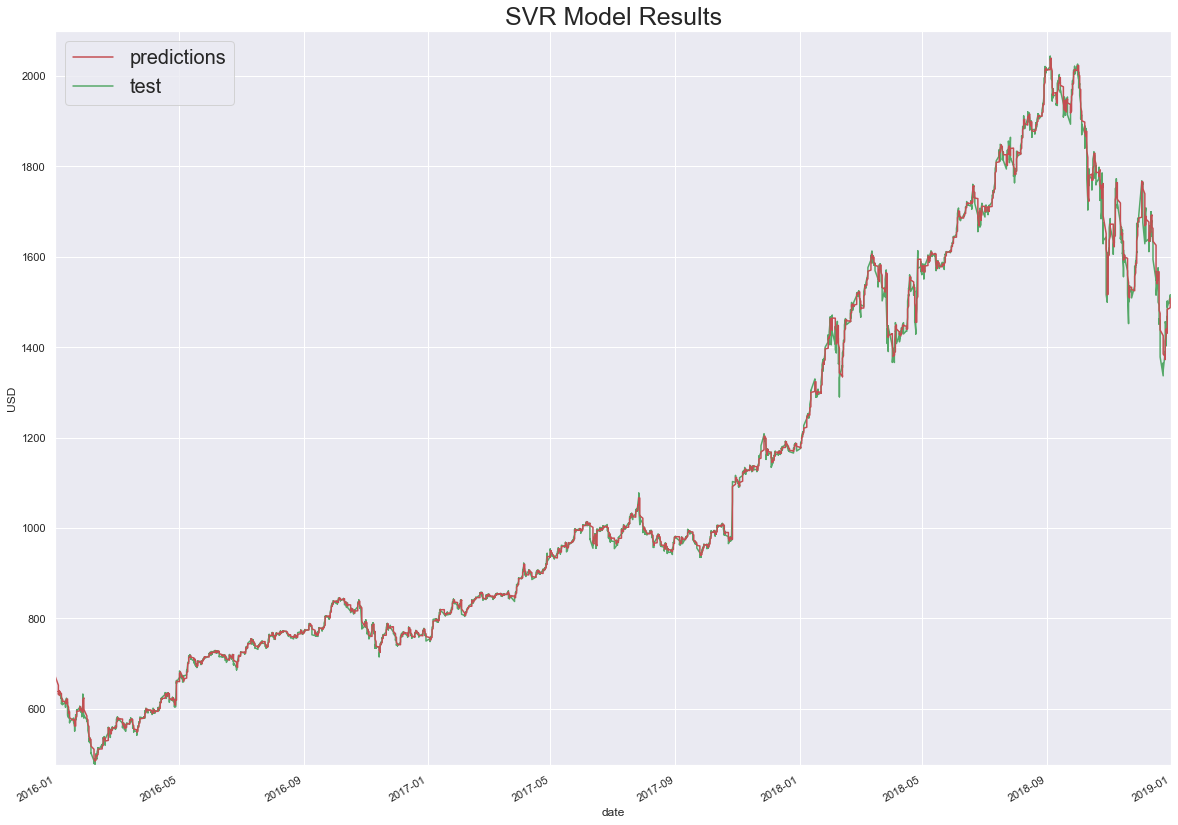
\includegraphics[width=1.5in]{SVR_amazon.png}
        \label{fig:second_sub}
    }
    \subfigure[Google]
    {
        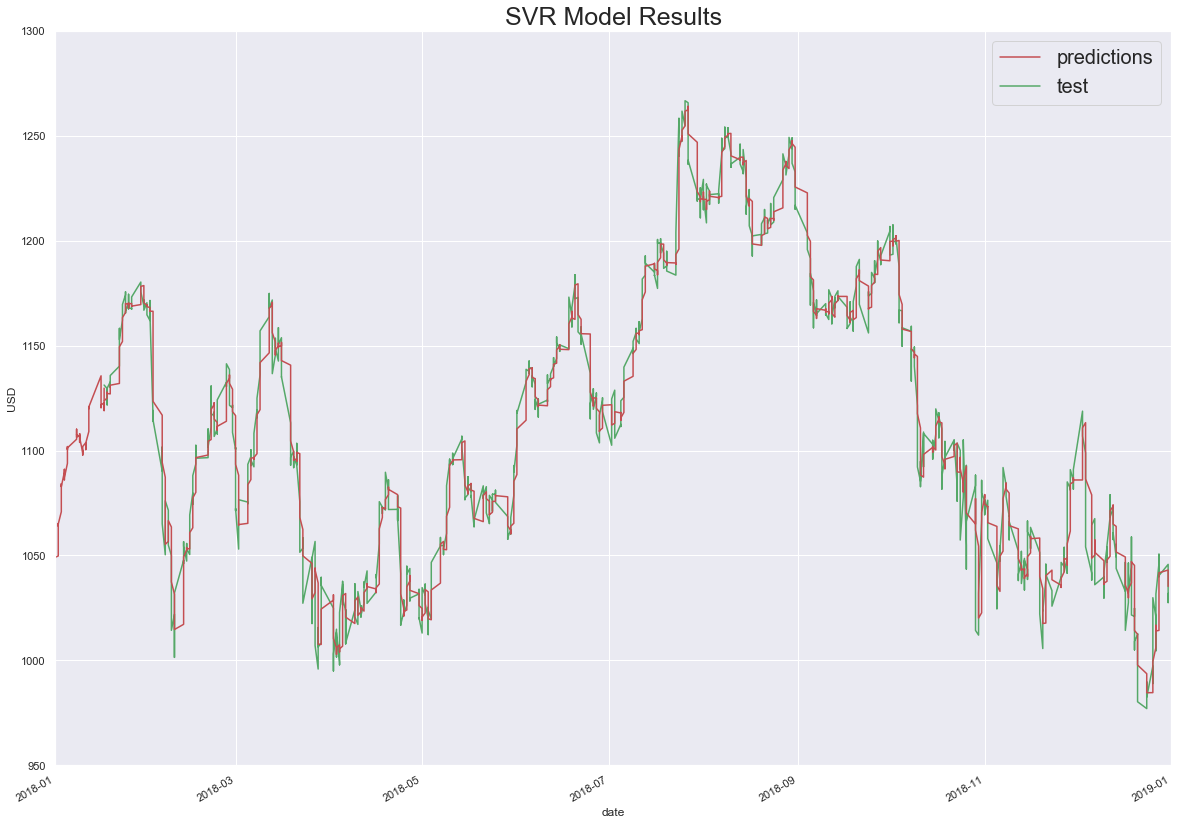
\includegraphics[width=1.5in]{srv_google.png}
        \label{fig:second_sub}
    }
    \subfigure[Microsoft]
    {
        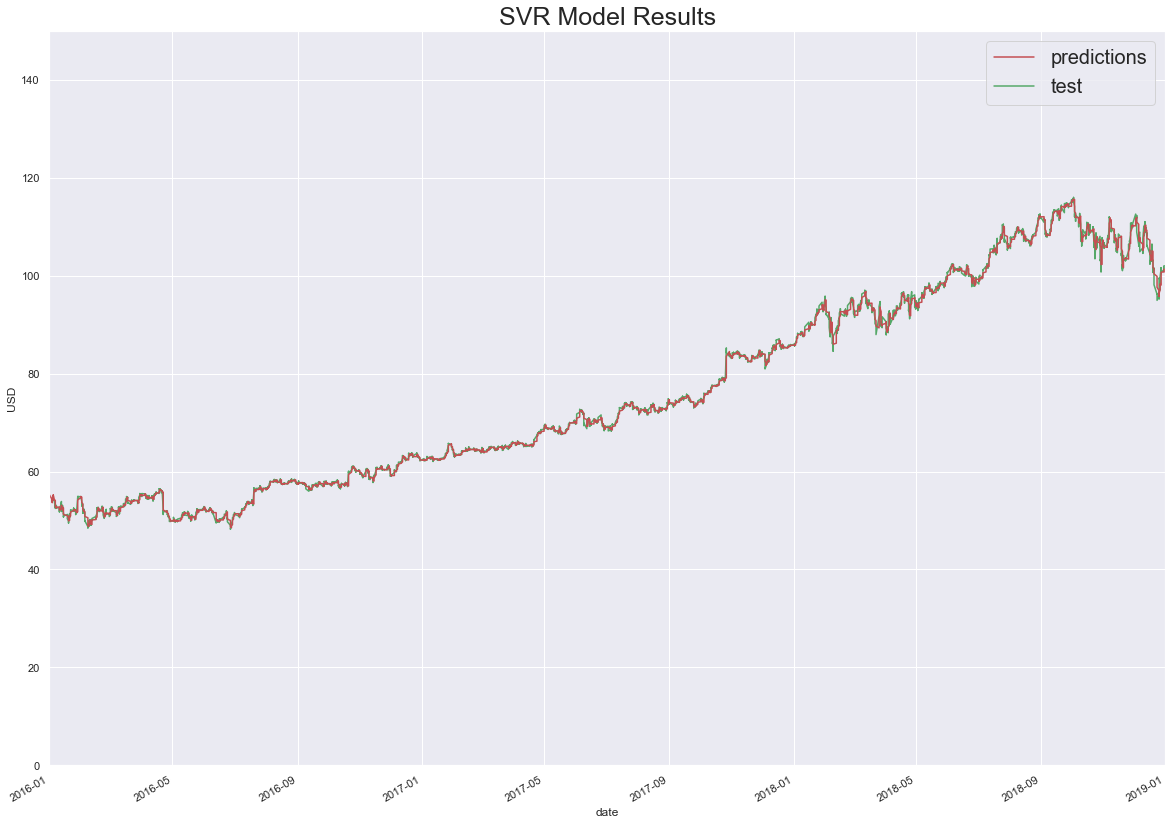
\includegraphics[width=1.5in]{SVR_micro.png}
        \label{fig:second_sub}
    }
    \caption{SVR Model Results for the Big 5 Tech Companies}
    \label{fig:sample_subfigures}
\end{figure}
\\
\\


\subsection{Support Vector Machine (SVM)}
Support Vector Machines are one of the best binary classifiers. They create a decision boundary such that most points in one category fall on one side of the boundary while most points in the other category fall on the other side of the boundary. Consider an n-dimensional feature vector $x = (X_1,...,X_n)$ \cite{8}. We can define a linear boundary (hyperplane) as
\begin{equation}
   \beta_0+ \beta_1 X_1+ ... + \beta_m X_m= \beta_0 + \sum_i ^n \beta_i X_i =0. 
\end{equation}
Then elements in one category will be such that the sum is greater than 0, while elements in the other category will have the sum be less than 0. With labeled examples, $ \beta_0 + \sum_i ^n \beta_i X_i =y$, where $y$ is the label. In our classification, $y \epsilon \{-1, 1\}$. We can rewrite the hyperplane equation using inner products.

\begin{equation}
  y= \beta_0 + \sum_i ^n \alpha_i y_i x(i).x
\end{equation}
where $.$ represents the inner product operator. Note that the inner product is weighted by its label. The optimal hyperplane is such that we maximize the distance from the plane to any point. This is known as the margin. The maximum margin hyperplane (MMH) best splits the data. However, since it may not be a perfect differentiation, we can add error variables $\epsilon_1 ...\epsilon_n$ and keep their sum below some budget B. The crucial element is that only the points closest to the boundary matter for hyperplane selection; all others are irrelevant. These points are known as the \textit{support vectors}, and the hyperplane is known as a Support Vector Classifier (SVC) since it places each support vector in
one class or the other.
The concept of the SVC is similar to another popular linear regression model, Ordinary Least Squares (OLS), but the two optimize different quantities. The OLS finds the residuals, the distance from each data point to the fit line, and \textit{minimizes} the sum of squares of these residuals \cite{9}. The SVC on the other hand looks at only the support vectors, and uses the inner product to \textit{maximize} the distance from hyperplane to the support vector. Additionally, the inner products in SVC are weighted by their labels, whereas in OLS the square of residuals serves as the weighting. A linear classification in the higher-dimensional space will be non-linear in the original space. The SVM replaces the inner product with a more general kernel function K which allows the input to be mapped to higher-dimensions. Thus in an SVM,

\begin{equation}
  y= \beta_0 + \sum_i ^n \alpha_i y_i K(x(i),x)
\end{equation}
The specific kernel function we use in this study is the radial kernel. This function is one of the most popular kernel functions and is defined as
\begin{equation}
K(x_i,x_j)=e^{-\frac{\sum_{\alpha=1} ^n (x_{i\alpha}-x_{j\alpha})^2}{\delta^2}}
\end{equation}
where $\delta$ is known as the bandwidth of the kernel function \cite{10}. The advantage of this function is that it can handle diverse input sets, as there are “few conditions on the geometry” of the input data \cite{11}. Additionally, it classifies test examples based on the example’s Euclidean distance to the training points, and weights closer training points more heavily. This means that classification is based heavily on the most similar training examples and takes advantage of patterns in the data. This is exactly what is needed for time-series data such as stock prices that display trends. We use the python library sklearn’s implementation of SVM.
\subsubsection{Feature Selection}
In this study we use four features to predict stock price direction – price volatility, price momentum. However in order to have a better comparison with other methods we used \textit{High - Low} prices and \textit{Open - Close}. 

In Table \ref{SVM_TAb} we describe how each of the four features are calculated by averaging some quantity over the past n hours. We conduct our study by varying this parameter n to see exactly how trends in volatility and momentum, both of the particular stock and the index, can be used to predict future changes in that stock.

\begin{table}[ht]\label{tab:SVM_TAb}
\centering
\caption{Features used in SVM}
\begin{tabular}[t]{lcc}
\hline
Feature name &  Formula\\
\hline
$\sigma_s$&$\frac{1}{n}\sum_{j=t-n+1}^{t} \frac{C_j-C_{j-1}}{C_{j-1}}$\\
Stock Momentum &$\frac{1}{n}\sum_{j=t-n+1}^{t} y_j$\\
High-Low&High price - Low price\\
Open-Close& Open price - Close price
\hline
\end{tabular}

\end{table}%
In the table \ref{tab:SVM_TAb},  stock price volatility. This is an average over the past n hours of percent change in the given stock’s price per hour and This is an average of the given stock’s momentum over the past n hours. Each hour is labeled 1 if closing price that hour is higher than the hour before, and −1 if the price is lower than the hour before.
\\
We are calculating the features to try and predict the price direction m hours in the future, where $m \epsilon \{ 5, 10, 50, 100\}$.
\\
We also have a set of output vectors y. y is calculated by finding the price direction on each of the 2014 − d − m hours. We then split $X$ and $Y$ into the training and testing sets as described before, which we call $X_{train}$, $y_{train}$, $X_{test}$, $y_{test}$. We supply the feature vectors $X_{train}$ as well as their corresponding output vectors $y_{train}$ to the SVM model. This is the training phase. We then supply only the testing feature vectors $x_{train}$ and have the model predict their corresponding output vectors. We then compare this output to $y_{train}$.
\subsubsection{Discussion}
One notable result is that the SVM model is only tenths of a percentage point better than simple random guessing when it comes to predicting price direction one hour ahead (m = 1). This has several important implications. First, it strongly reinforces the Efficient Markets Hypothesis. If a model that incorporates several types of historical data, including some features like momentum that economists have demonstrated are present in stock price data, is not able to do better than a coin flip when it comes to predicting the next hour’s price direction, then this is very strong evidence that prices follow a random walk. Prices that already reflect available information will change only based on new information, so next hours’s price direction will be dependent only on new information that arrives tomorrow. A model like ours which analyzes only historical data should not be able to predict the price direction, as all this historical data should already be incorporated into the price. Therefore, our model’s difficulty in predicting the next hour’s stock price supports EMH.
\\
Several trends emerge as we increase the parameter m. The most striking is that the mean and median returns increase when m = 5, 10 but then decrease slightly when m = 50 and m = 100. Figure \ref{fig:SVM} shows the mean prediction accuracy against the parameter m, where mean prediction accuracy here is the mean of the mean accuracies for all 25 combinations of $n_1,n_2$ with a fixed m, where each combination itself reports the mean accuracy across the 34 stocks.
\begin{figure}[t]\label{fig:SVM}
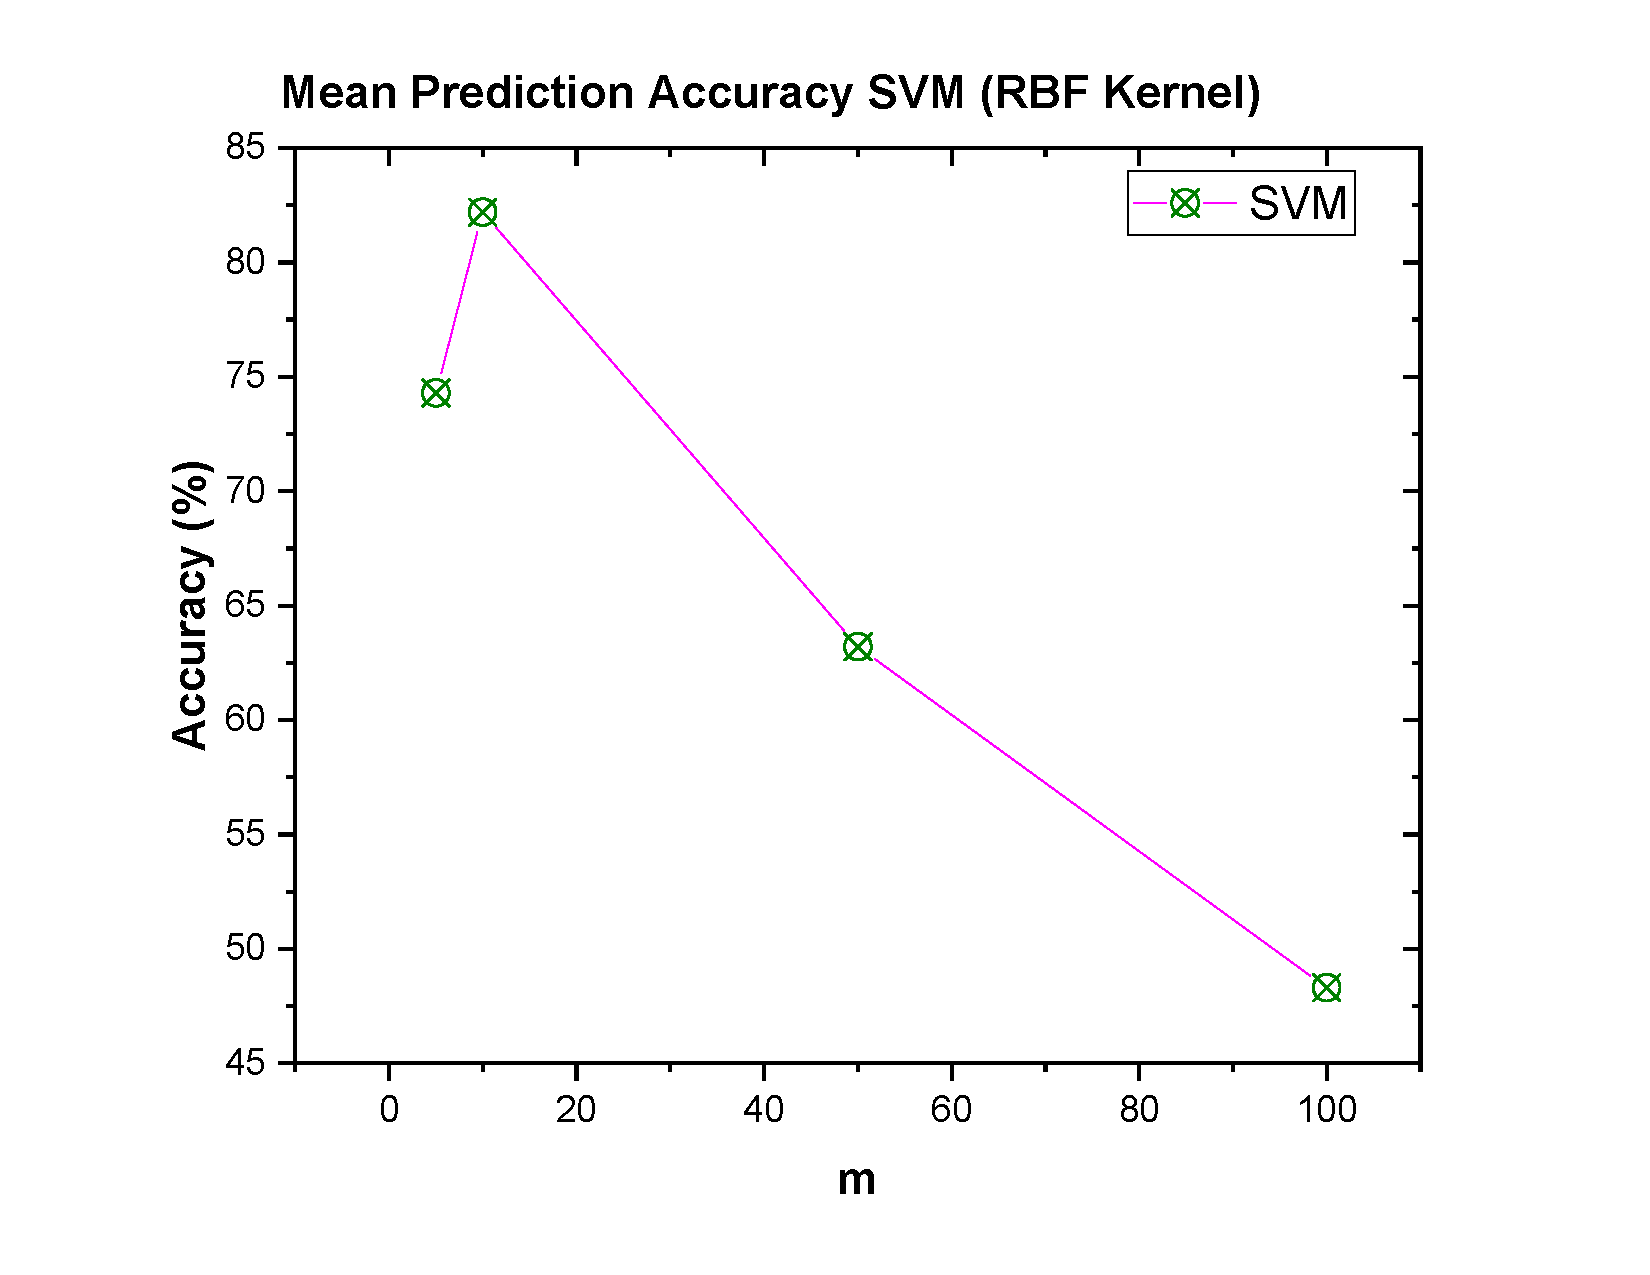
\includegraphics[width=8cm]{SVM_1.pdf}
\centering
\caption{The mean prediction accuracy for each parameter m.}
\end{figure}




\subsection{Long Short-Term Memory (LSTM)}

Long short-term memory (LSTM) is an artificial recurrent neural network (RNN) architecture[1] used in the field of deep learning. Unlike standard feedforward neural networks, LSTM has feedback connections. It can not only process single data points (such as images), but also entire sequences of data (such as speech or video).  

A common LSTM unit is composed of a cell, an input gate, an output gate and a forget gate. The cell remembers values over arbitrary time intervals and the three gates regulate the flow of information into and out of the cell. LSTM networks are well-suited to classifying, processing and making predictions based on time series data, since there can be lags of unknown duration between important events in a time series. From below figure we can see the simplified structure: 


\begin{figure}[htpb]
\begin{center}
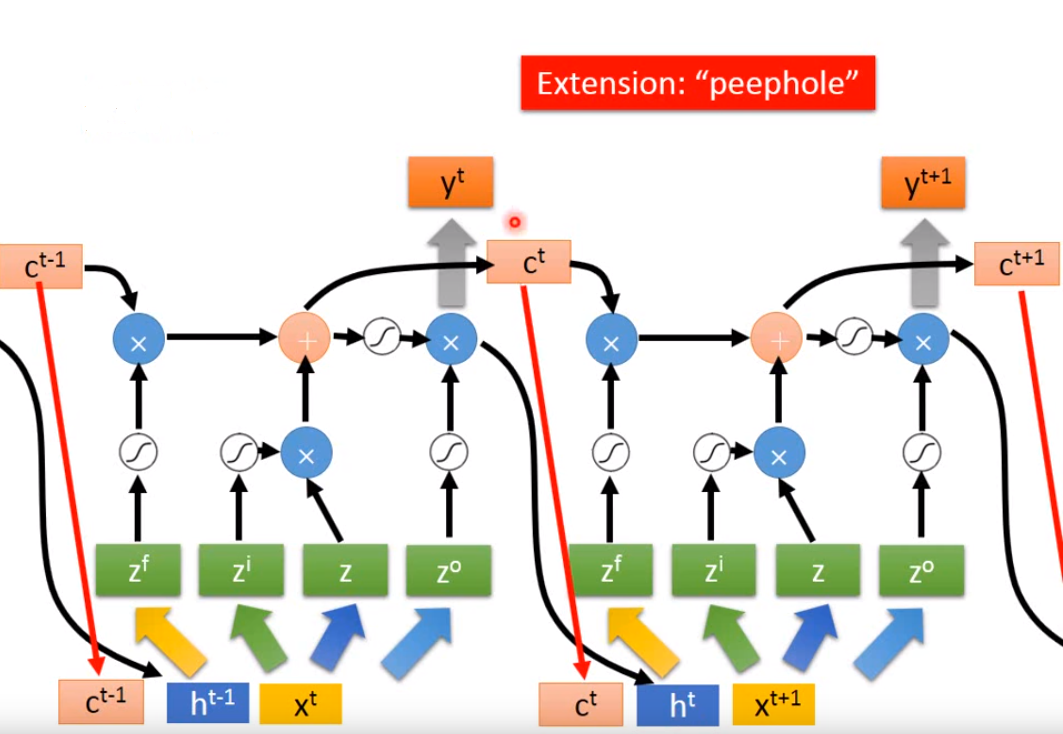
\includegraphics[width=0.35\textwidth]{LSTM_source/LSTM_1.PNG}
\vspace{-0.2cm}
\caption{Simplified Long Short-Term Memory (LSTM) structure \cite{12}}
\label{fig_bar}
\end{center}
\vspace{-0.4cm}
\end{figure}

Stock market prediction is usually considered as one of the most challenging issues among time series predictions ~\cite{13} because of its volatile properties. Here we try to do experiments on an improved model which models complex real-world data by extracting robust features that capture the relevant information. Considering the complexity of financial time series, neural network is regarded as one of the most charming topic. Surprisingly, the application of LSTM in financial area has yet been little and there has not been any previous attempt to deploy LSTM networks on a large, liquid, and survivor-bias-free stock universe to assess its performance in large-scale financial market prediction tasks [5]. Unlike conventional RNN, LSTM is well-suited to learn from experience to predict time series when there are time steps with arbitrary size.  In addition, it can solve the problem of a vanishing gradient by having the memory unit retain the time related information for an arbitrary amount of time  [7]. Previous work has shown that LSTM is more effective than RNN.  
\\ 
\\
Below is a peephole LSTM unit with input (i.e. ), output (i.e. ), and forget (i.e. ) gates. Each of these gates can be thought as a "standard" neuron in a feed-forward (or multi-layer) neural network: that is, they compute an activation (using an activation function) of a weighted sum. and represent the activations of respectively the input, output and forget gates, at time step . The 3 exit arrows from the memory cell to the 3 gates and represent the peephole connections. These peephole connections actually denote the contributions of the activation of the memory cell at time step , i.e. the contribution of (and not , as the picture may suggest). In other words, the gates and calculate their activations at time step (i.e., respectively, and ) also considering the activation of the memory cell at time step , i.e. . The single left-to-right arrow exiting the memory cell is not a peephole connection and denotes . The little circles containing a symbol represent an element-wise multiplication between its inputs. The big circles containing an S-like curve represent the application of a differentiable function (like the sigmoid function) to a weighted sum. There are many other kinds of LSTMs as well.[5]

\begin{figure}[htpb]
\begin{center}
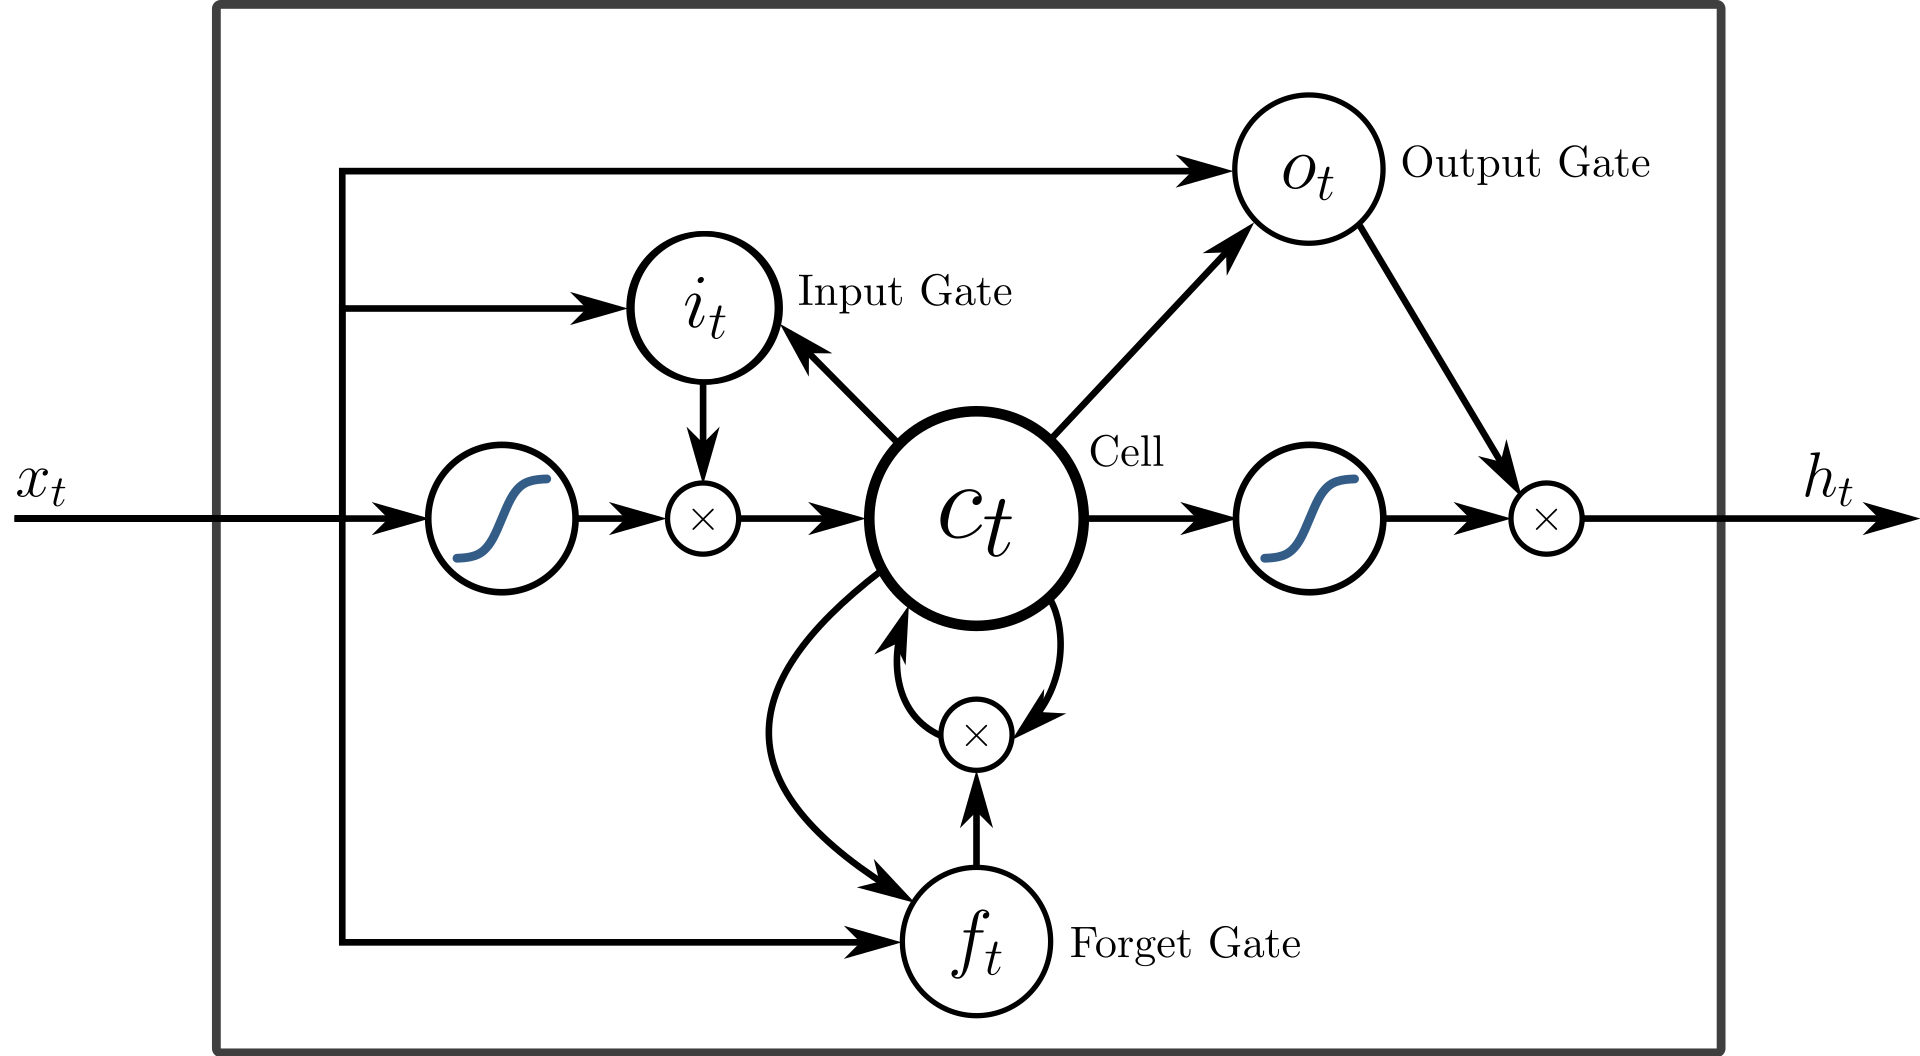
\includegraphics[width=0.35\textwidth]{LSTM_source/LSTM_2.png}
\vspace{-0.2cm}
\caption{A peephole LSTM unit \cite{14}}
\label{fig_bar}
\end{center}
\vspace{-0.4cm}
\end{figure}


There are six features being employed in the network. There are "Weighted AVG. PRICE", "VOLUME", "OPEN", "CLOSE", "HIGH", "LOW". And also we tested top 5 tech companies' stock history data. 

About software and hardware. Since we didn't successfully secure a powerful GPU (though we have one on Thinkpad laptop machine, it is very slow), we choose to run the cold on Macintosh computer with i5 core CPU. Data preparation and handling are entirely conducted in Python 3.7 (Python Software Foundation,2018), relying on the packages NumPy (Van Der Walt, Colbert,  Varoquaux, 2011), Pandas (McKinney,2010). The neural network with LSTM are developed with keras (Chollet, 2016) on top of GoogleTensorFlow, a powerful library for large-scale machine learning on heterogenous systems (Abadi etal., 2015).  

Since our computer's power is limited, we only test each stock with 2, 5 and 10 epoch. As the epoch going larger, the accuracy goes from 55\% to 70\%. And we test the loss with RMSE, MAPE, MSE, and MAE


\begin{table}[h]
\renewcommand{\arraystretch}{1.3}
\caption{Calculated Metrics (LSTM)}
\label{tab:example}
\centering


\begin{tabular}{|c|c|c|c|c|c|}
    \hline
    Stocks  &  RMSE & MSE & MAE & MAPE(\%) \\
    \hline
    \hline

    Apple   &   0.00508 & 2.58834 & 0.003023 & 0.831  \\
    \hline

    Facebook   &   2.4062 & 5.7898 & 1.4136 & 0.8412  \\
    \hline

    Google   &  0.004826  & 2.329 & 0.00280  & 0.8338is i  \\
    \hline
  
    Amazon   &  0.00687  & 4.726  & 0.0451 & 0.82686  \\
    \hline
    
    Microsoft   &  0.00728  & 5.3073 & 0.00498 & 0.8235  \\
    \hline
\end{tabular}

\end{table}

Below are some of the result figures for each index.  

\begin{figure}[htpb]
\begin{center}
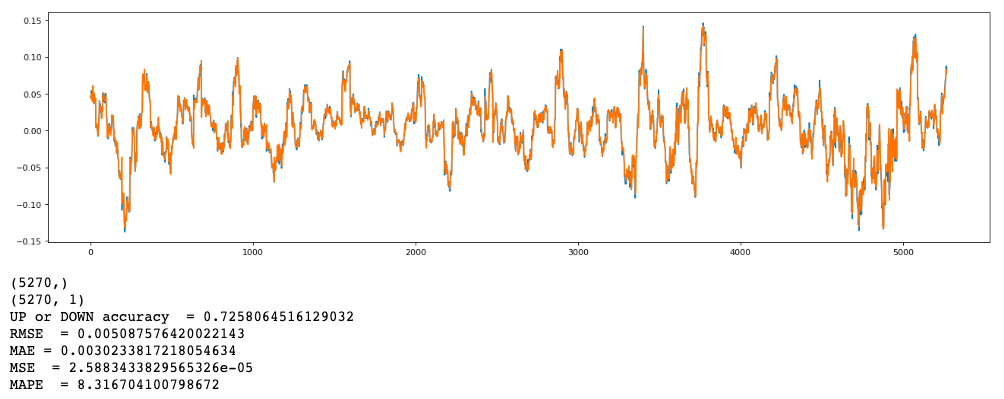
\includegraphics[width=0.45\textwidth]{LSTM_source/LSTM_10_Apple.png}
\vspace{-0.2cm}
\caption{Apple stock prediction; 10 epochs; Up/Down Accuracy: 72.5\%}
\label{fig_bar}
\end{center}
\vspace{-0.4cm}
\end{figure}

\begin{figure}[htpb]
\begin{center}
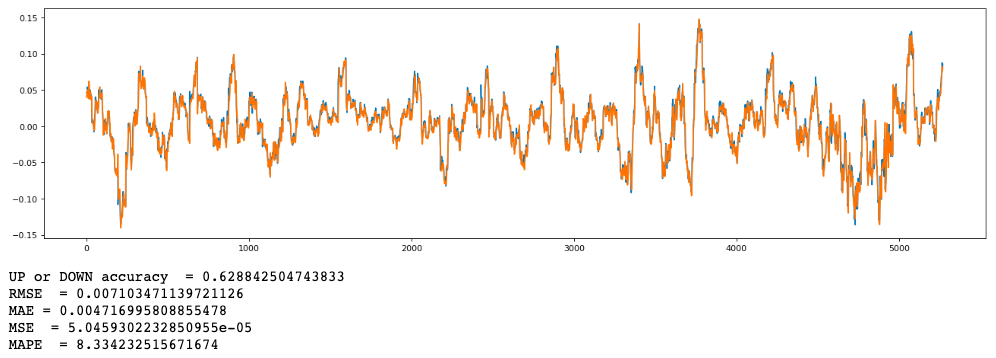
\includegraphics[width=0.45\textwidth]{LSTM_source/LSTM_10_Facebook.png}
\vspace{-0.2cm}
\caption{Facebook stock prediction; 5 epochs; Up/Down Accuracy: 62.5\%}
\label{fig_bar}
\end{center}
\vspace{-0.4cm}
\end{figure}

\begin{figure}[htpb]
\begin{center}
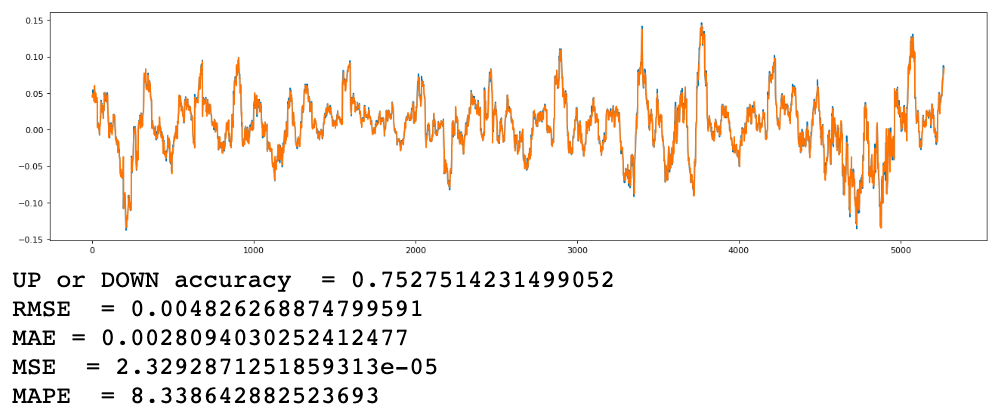
\includegraphics[width=0.45\textwidth]{LSTM_source/LSTM_10_Google.png}
\vspace{-0.2cm}
\caption{Google stock prediction; 10 epochs; Up/Down Accuracy: 75\%}
\label{fig_bar}
\end{center}
\vspace{-0.4cm}
\end{figure}
 
Also, we did some test for closer look at the prediction with point to point for 50 hours. And also sequence by sequence for 50 hours too. Please refer to figure 13-17.


\begin{figure}[htpb]
\begin{center}
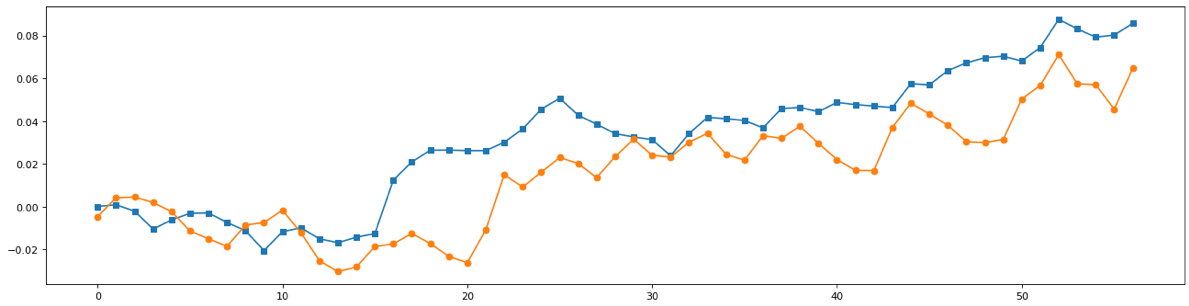
\includegraphics[width=0.45\textwidth]{LSTM_source/PP_2_50.PNG}
\vspace{-0.2cm}
\caption{Point-by-Point prediction (2 Epoch, 50 Batch size)}
%\todo{fix scale from 1 to 41 and 1 to 100}}
\label{fig_predict}
\end{center}
\vspace{-0.6cm}
\end{figure}

\begin{figure}[htpb]
\begin{center}
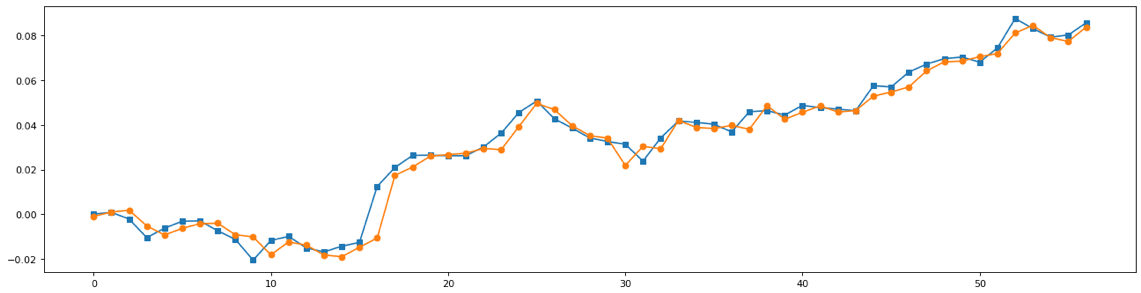
\includegraphics[width=0.45\textwidth]{LSTM_source/PP_8_50.PNG}
\vspace{-0.2cm}
\caption{Point-by-Point prediction (8 Epoch, 50 Batch size)}
%\todo{fix scale from 1 to 41 and 1 to 100}}
\label{fig_predict}
\end{center}
\vspace{-0.6cm}
\end{figure}

\begin{figure}[htpb]
\begin{center}
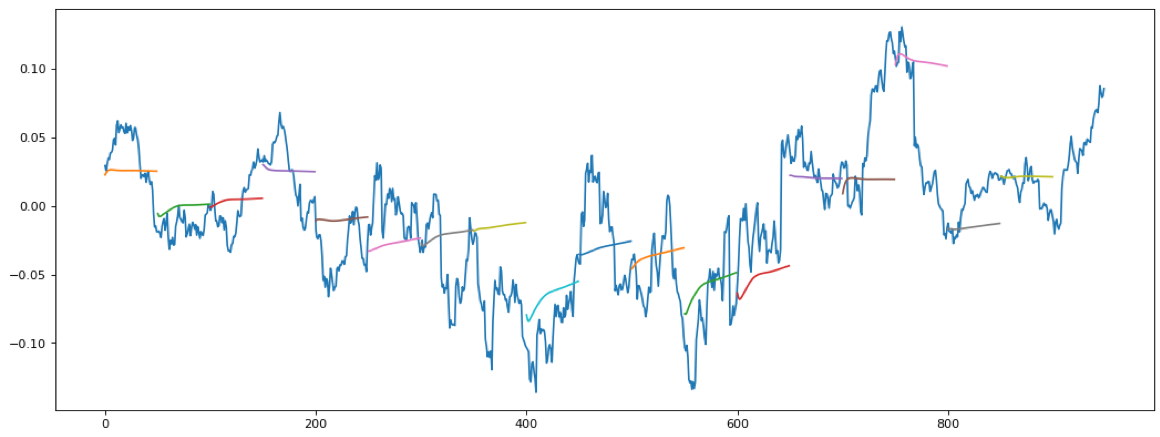
\includegraphics[width=0.45\textwidth]{LSTM_source/SS_2_50.PNG}
\vspace{-0.2cm}
\caption{Sequence-by-Sequence prediction (2 Epoch, 50 Batch size)}
%\todo{fix scale from 1 to 41 and 1 to 100}}
\label{fig_predict}
\end{center}
\vspace{-0.6cm}
\end{figure}

\begin{figure}[htpb]
\begin{center}
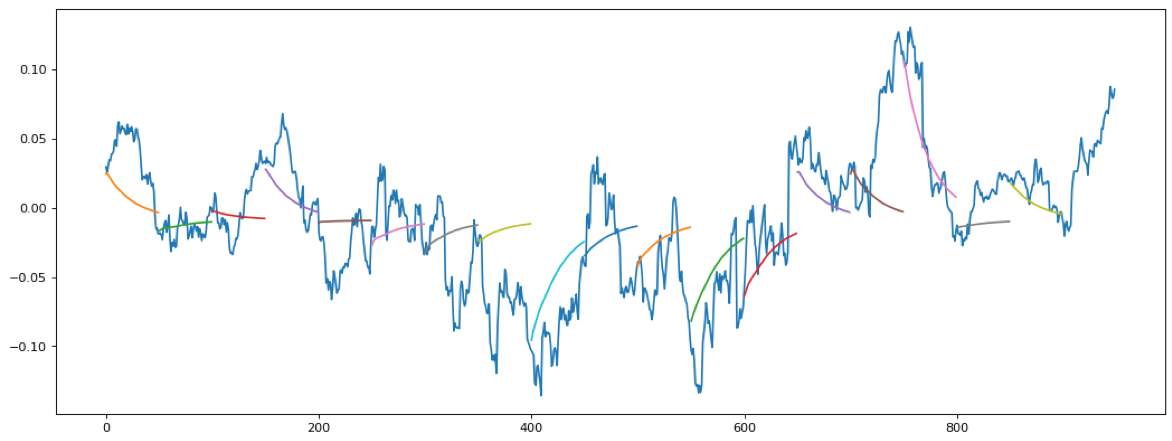
\includegraphics[width=0.45\textwidth]{LSTM_source/SS_4_50.PNG}
\vspace{-0.2cm}
\caption{Sequence-by-Sequence prediction (4 Epoch, 50 Batch size)}
%\todo{fix scale from 1 to 41 and 1 to 100}}
\label{fig_predict}
\end{center}
\vspace{-0.6cm}
\end{figure}




\section{DISCUSSION}
THE SVR model performed relatively well. It performed best for the companies we had the most amount of data for: Apple, Facebook, and Microsoft. It did not do so well for Google and Amazon which had less data and are data sets that are much more varied. It seems that when the data is stable, the SVR can perform quite well. When the data is varied with large increases and decreases in stock, the SVR model does not adjust well, and cannot predict prices nearly as well. One of the main benefits of the SVR model is the fact that it is a very quick method. Optimizing the parameters takes some time, but training and running the model on the test data takes hardly any time at all. Considering the speed of the SVR, the overall performance on prediction is good.  

\\
\\
For comparative study of the supervised learning algorithms for stock market prediction, accuracy and F-measure are used in this paper. Accuracy is mathematically expressed using equation (1) and F-measure is mathematically expressed by equation (2), where TP is true positive, TN is true negative, FP is false positive and FN is false negative
\begin{equation}
    Accuracy= \frac{TP-TN}{TP+TN+FP+FN}
\end{equation}
The results evaluated for four indicators are shown in Table below and for four methods.


\begin{table}[]
\begin{center}
 \begin{tabular}{||c | c c c||} 
 \hline
 Methods & RMSE & MAE & MAPE \\ [0.5ex] 
 \hline\hline
LTSM & - & - & - \\ 
 \hline
SVM & 0.742 & 0.442 & 0.293 \\
 \hline
XGboost & 0.837 & 0.474 & 0.305 \\
 \hline
SVR & 1.468 & 0.9351 & 0.6018 \\
 \hline
\end{tabular}
\end{center}
    \caption{Loss functions for Apple hourly data from 2004-2019. RMSE:Root Mean Square Error, MAE: Mean Absolute Error, MAPE: Mean Absolute Percentage Error. }
    \label{tab:my_label}
\end{table}





\section{CONCLUSION}
In this project, we have demonstrated a machine learning approach to predict the stock market trend using supervised and different neural networks. The result shows how we can use historical data to predict stock movement with reasonable accuracy. Also, with XGboost result analysis we can conclude that LSTM performs better compare to Linear regression and SVM. For this implementation, we would like to conclude that if I incorporate all the factors that affect stock performance and feed them to neural network with proper data preprocessing and filtering, after training the network we will be able to have a model which can predict stock momentum very accurately and this can result into better stock forecasting and profit for financial firms.

\section{Future Work}
Feature selection often has the biggest impact on a machine learning model’s accuracy. Another area for future work is to add to our feature list. Here we have looked at price High-low and Rolling mean and  momentum and Rolling std for the particular stock and for the technology sector which apple INC. Future work would involve adding features related to the specific company and related to broader macroeconomic factors. Features related to the specific company include its Price/Earnings ratio, its market cap, working capital ratio, cost-of-capital, etc. Features related to broader factors include interest rate, inflation, GDP growth rate, etc.

\section{Repository}
GITHUB:\\
\url{https://github.com/faisalkhan1994/Machine-Learning}

\section*{Acknowledgment}
We would like to thank Dr. Bobak Mortazavi for his contributions to our understanding and the relevant background knowledge needed in order to successfully implement the information discussed throughout this paper. We would also like to thank Arash Pakbin for his guidance and advice. Lastly, we would like to thank our classmates who offered their advice and support throughout the entire course that aided in our understanding of the material.

\begin{thebibliography}{1}
\bibitem{1} 
Carson Kai-Sang Leung, Richard Kyle MacKinnon, and Yang Wang. 2014. A machine learning approach for stock price prediction. In Proceedings of the 18th International Database Engineering \& Applications Symposium (IDEAS '14), Ana Maria Almeida, Jorge Bernardino, and Elsa Ferreira Gomes (Eds.). ACM, New York, NY, USA, 274-277. DOI: \url{https://doi.org/10.1145/2628194.2628211}
 
\bibitem{2} 
Biao Huang, Qiao Ding, Guozi Sun, and Huakang Li. 2018. Stock Prediction based on Bayesian-LSTM. In Proceedings of the 2018 10th International Conference on Machine Learning and Computing (ICMLC 2018). ACM, New York, NY, USA, 128-133. DOI: \url{https://dl.acm.org/citation.cfm?id=3195170}

\bibitem{3}
scikit-learn.org, 'RBF SVM parameters', 2014. Available: \url{https://scikit-learn.org/stable/auto_examples/svm/plot_rbf_parameters.html}. [Accessed: 29- Nov- 2019].

\bibitem{4}
saedsayad.com, 'Support Vector Machine - Regression (SVR)', 2014. Available: \url{https://www.saedsayad.com/support_vector_machine_reg.htm.} [Accessed: 29- Nov- 2019].

\bibitem{5}
Stock Prediction with XGBoost: A Technical Indicators’ approach: \url{https://medium.com/@hsahu/stock-prediction-with-xgboost-a-technical-indicators-approach-5f7e5940e9e3}

\bibitem{6}
Forecasting Stock Prices using XGBoost: \url{https://towardsdatascience.com/forecasting-stock-prices-using-xgboost-a-detailed-walk-through-7817c1ff536a}

\bibitem{7}
XGBoost Parameters:
\url{https://xgboost.readthedocs.io/en/latest/parameter.html}

\bibitem{8}
M. Halls-Moore, “Support vector machines: A guide for beginners,” September 2014. [Online]. Available:
\url{http://www.quantstart.com/articles/Support-Vector-Machines-A-Guid e-for-Beginners}
\bibitem{9}
M. W. W. James H. Stock, Introduction to Econometrics. Addison-Wesley, 2015.
\bibitem{10}
K.jae Kim,“Financial time series forecasting using support vector machines,” \textit{Neurocomputing}, vol.55, 2003.

\bibitem{11}
M. Buhmann, “Radial basis function.” Mathematisches Institut, Justus-Liebig-Universität Giessen, 2010.

\bibitem{12}
Hung-yi Lee, “ML Lecture 21-1: Recurrent Neural Network (Part I)”, https://youtu.be/xCGidAeyS4M
 
\bibitem{13}
B. Wang, H. Huang, and X. Wang.   A novel text mining approach to financial time seriesforecasting.Neurocomputing, 83:136–145, 2012.

\bibitem{14}
A peephole LSTM unit with input, output, and forget   gates,  \url{https://en.wikipedia.org/wiki/Long_short-term_memory}


\bibitem{15}
Bao, Wei, Jun Yue, and Yulei Rao. "A deep learning framework for financial time series using stacked autoencoders and long-short term memory." PloS one 12, no. 7 (2017): e0180944.

\end{thebibliography}




%\bibliographystyle{plain}
%\bibliographystyle{abbrv}
%\bibliographystyle{abbrvnat}
%\bibliographystyle{ACM-Reference-Format}
%\bibliography{Final_report}


\end{document}
